\clearpage
\chapter{Background Estimation}\label{sec:estimate}

Section ~\ref{sec:selections} listed seven different discriminant variables for the analysis.
Leading ROI score, subleading ROI score, and leading muon's IP value have the most discriminatory power.
The analysis uses data-driven background estimation method and an ABCD method is the most preferred thanks to its simplicity.
However, leading ROI score and subleading ROI score are correlated in the QCD background process.
ROIs from B-mesons score higher in our tensorflow.
In QCD processes, the B-mesons are likely to be pair produced.
Therefore, when the leading ROI score is high due to its b-like behavior, the sublead ROI score is also high because the anti-meson is produced on the other side of the detector.
Thus, leading and sublead scores can't be our ABCD discriminant variable candidates du to their correlation.

The analysis selects leading ROI and leading muon's IP value as its ABCD discriminant variables.
After implementing all other cuts (sublead ROI, $\Delta\Phi(lead,sublead)$, Number of Annulus tracks associated with ROI, 1 Isolated $\mu$, $\Delta R(lead ROI, Jet)$), we tested the correlation factor between the leading ROI, and leading mu's IP values for each background process.
The values are pretty minimal except for 2-3 processes where there were too few entries to derive a physical conclusion due to statistical limitations.
Therefore, the analysis uses leading muIP and leading ROI score for its ABCD discriminant variables.

The results are listed below.  


 \begin{figure}[h!]
   \caption{Cutflow histogram of MS15GeV-ct100mm point. Left plot is for region A, whereas the right plot is for region D}
   \label{fig:ABmethod}
   \centering
   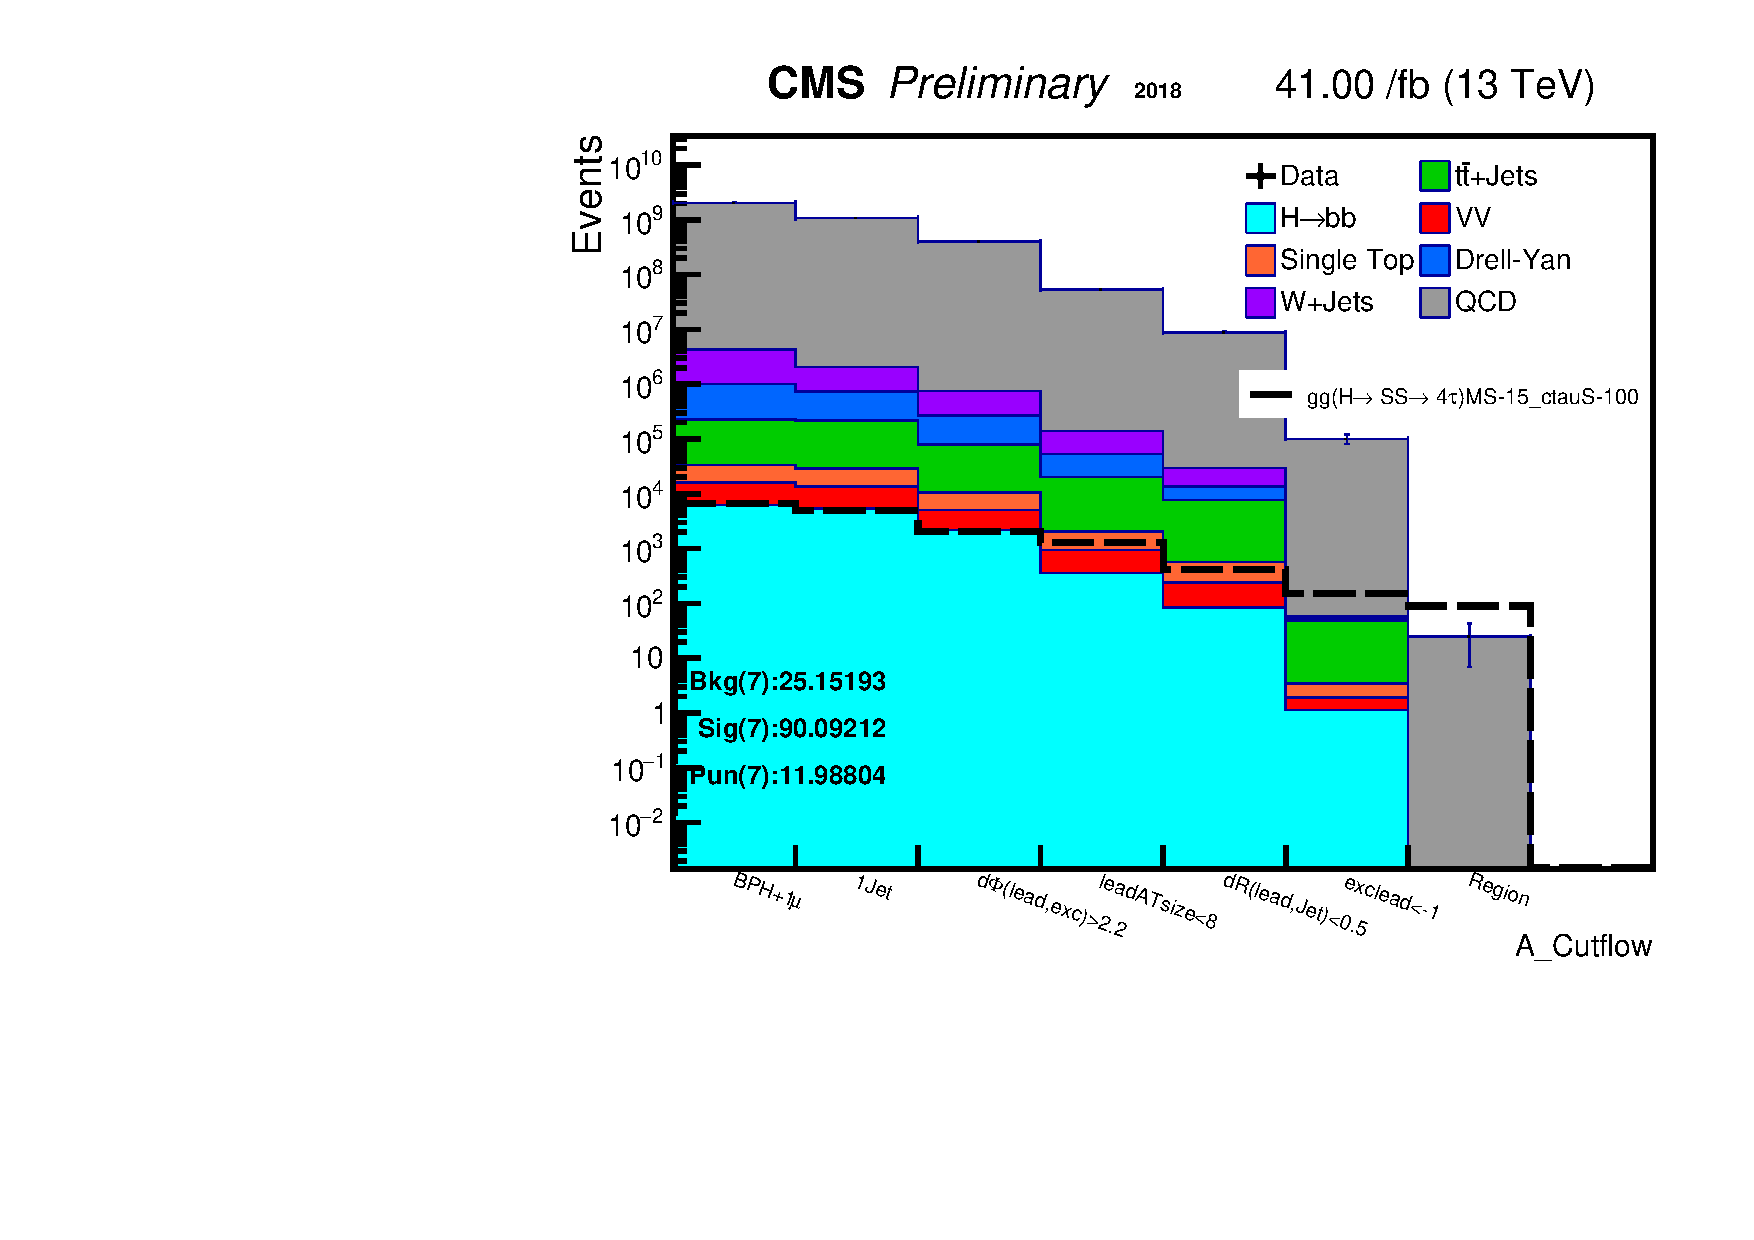
\includegraphics[width=0.47\linewidth]{figs/AnalysisNoteplot_MS-15_ctauS-100_A_Cutflow.pdf}
   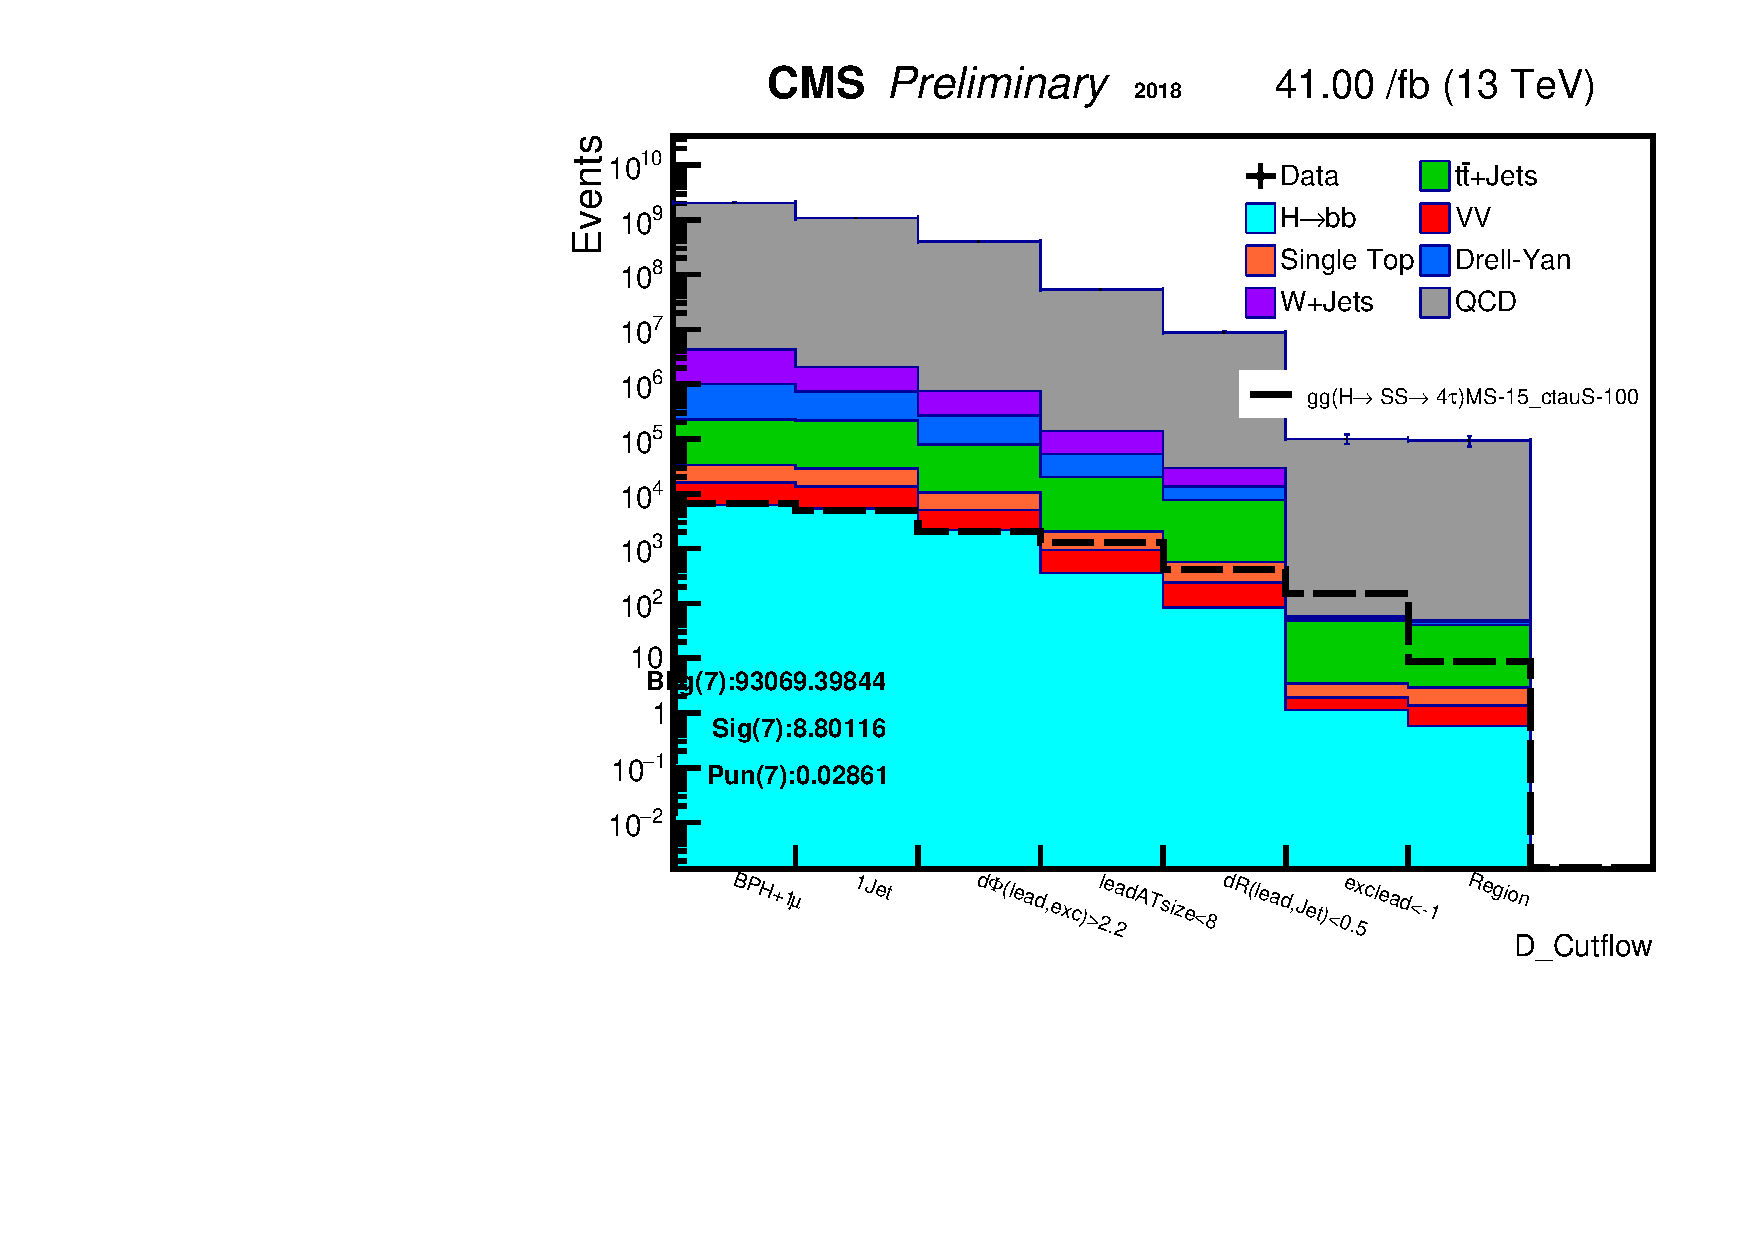
\includegraphics[width=0.47\linewidth]{figs/AnalysisNoteplot_MS-15_ctauS-100_D_Cutflow.pdf}
 \end{figure}

 \begin{figure}[h!]
   \caption{eee}
   \label{fig:ABCDmethod}
   \centering
   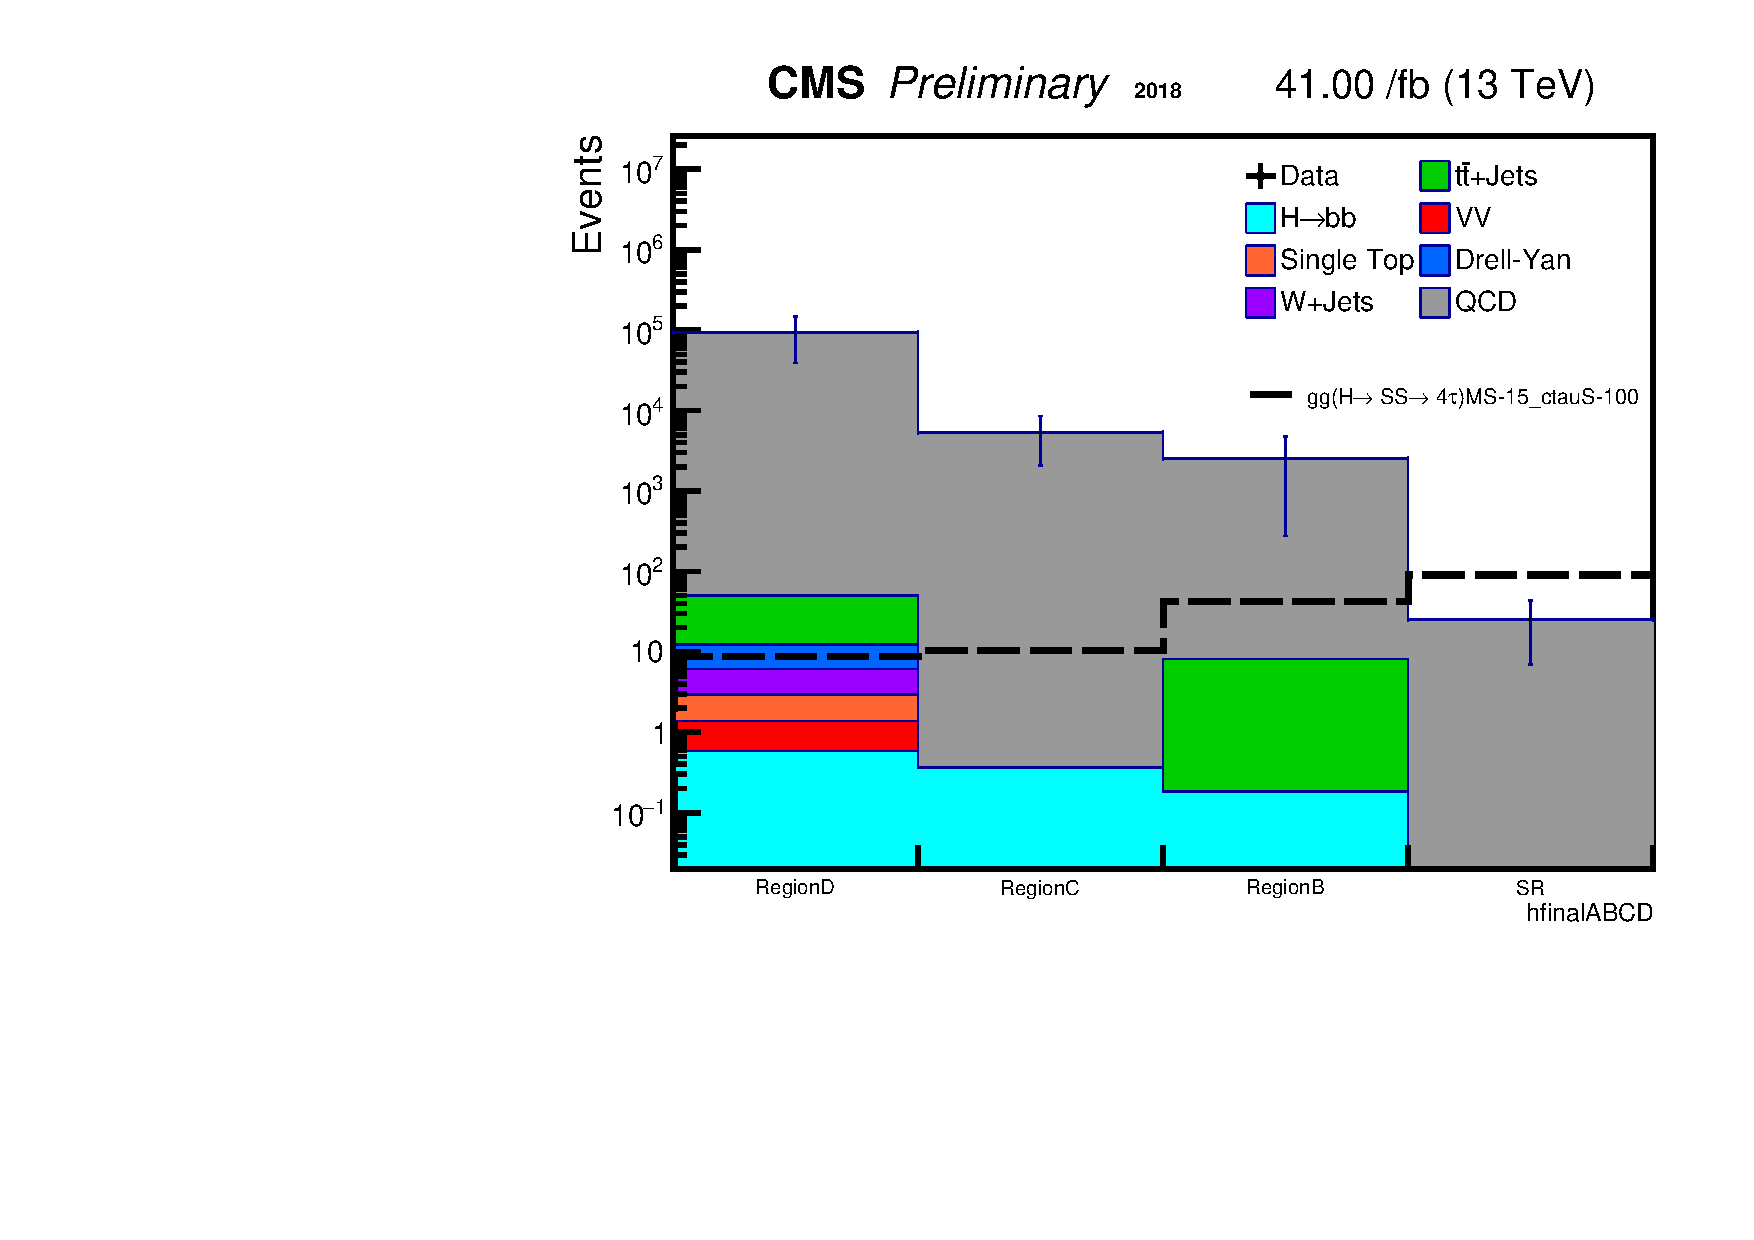
\includegraphics[width=0.67\linewidth]{figs/AnalysisNoteplot_MS-15_ctauS-100_hfinalABCD.pdf}
 \end{figure}
 
